\documentclass{beamer}
\usepackage[utf8]{inputenc}
\usepackage[croatian]{babel}
\usepackage{biblatex}
\usepackage{graphicx}
\addbibresource{literatura.bib}
\usetheme{Copenhagen}


\begin{document}

\title{Bibliografije}
\date{\today}
\author{Hana Rut Lerga \\ Anton Pavelić \\ Ivana Štimac}
\institute{Tehnički fakultet Rijeka}

\begin{frame}
\maketitle
\end{frame}

\begin{frame}
\tableofcontents
\end{frame}


\begin{frame}{Uvod}
\section{Uvod}
\begin{itemize}
	\item tri paketa za upravljanje bibliografijom:\\
	\begin{itemize}
		\item biblatex \\
		\item bibtex \\
		\item natbib \\
	\end{itemize}
\end{itemize}
	
\end{frame}

\begin{frame}{Biblatex\cite{biblatex}}
\section{Biblatex}
\begin{itemize}
	\item jedan od paketa za upravljanje bibloigrafijama \\
	\item jednostavno i moderno sučelje, lak za korištenje \\
	\item primjer korištenja: \\
	\begin{figure}
	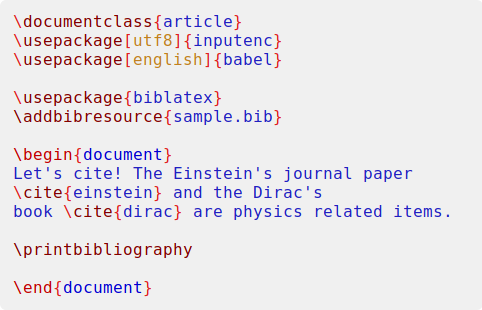
\includegraphics[width=5cm]{prviprimjer.png}
	\end{figure}
\end{itemize}
\end{frame}

\begin{frame}
\begin{itemize}
	\item paket se poziva naredbom \textbackslash usepackage\{biblatex\}\\
	\item \textbackslash cite je naredba kojom dodajemo referencu u tekst dokumenta \\
	\item \textbackslash printbibliography je naredba kojom se ispisuju reference \\
\end{itemize}
\end{frame}

\begin{frame}{Bibtex sintaksa}
\subsection{Biblatex sintaksa}
\begin{itemize}
	\item koristi se u svim navedenim paketima za upravljanje bibliografijama \\
	\item prvo se navodi na što se informacija koja se navodi u referenci odnosi \\
	\begin{itemize}
		\item @article\{...\} \\
		\item @book \{...\}\\
		\item @online \{...\} ... \\
	\end{itemize}
	\item ime reference, koristi se u tekstu kada se želi dodati određena referenca \\
	\item autor, naslov, godina... 
		\begin{itemize}
			\item primjer: year = 2010.
		\end{itemize}
\end{itemize}
\end{frame}

\begin{frame}{Parametri}
\begin{itemize}
	\item parametri, odnosno dodatne opcije, dodaju se unutar uglatih zagrada i odvajaju se zarezom \\
	\item može se mijenjati pozadina, stil (redoslijed referenci), način sortiranja... \\
	\item primjer:
	\begin{figure}
		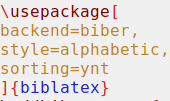
\includegraphics[width=2.5cm]{drugiprimjer.png}
	\end{figure}
\end{itemize}
\end{frame}

\begin{frame}{Dodavanje bibliografije u sadržaj}
\begin{itemize}
	\item dodatne opcije se upisuju pokraj \textbackslash printbibliography \\
	\item primjer:
	\begin{figure}
	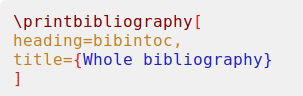
\includegraphics[width=5cm]{treciprimjer.png}
	\end{figure}
\end{itemize}
\end{frame}

\begin{frame}{BibTeX\cite{bibtex}}
\section{BibTex}
\begin{itemize}
    \item široko korišten paket za upravljanje bibliografijom \\
    \item podatke o bibliografiji može sadržavati u trenutnom 
    dokumentu ili u zasebnoj datoteci nastavka: .bib \\
    \item bibliografska datoteka stvara se pomoću već spomenute
    BibTex sintakse \\
\end{itemize}
\end{frame}

\begin{frame}{BibTex - u dokumentu}
\subsection{BibTex - u dokumentu}
\begin{itemize}
    \item primjer korištenja:
    \begin{figure}
    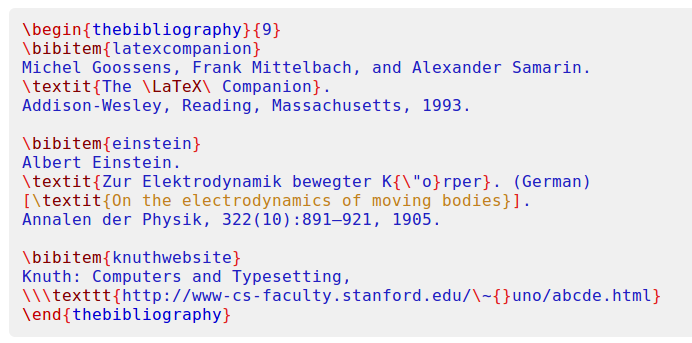
\includegraphics[width=10cm]{bibtexUDokumentu.png}
    \end{figure}
\end{itemize}    
\end{frame}

\begin{frame}
Objašnjenje naredbi:
\begin{itemize}
    \item \textbackslash begin\{thebibliography\}\{n\}:
        \begin{itemize}
            \item početak bibliografije \\
            \item n... broj navoda (literature); n \textless= 99 \\
        \end{itemize} \\
    \item \textbackslash bibitem\{ime\} - jedan navod; ime = referenca \\
    \item podatci o: autoru, naslovu, godini... \\
    \item \textbackslash end\{thebibliograhy\} - kraj bibliografije
\end{itemize}
Izgled:
\begin{itemize}
    \item stvara se lista referenci naslova \textbf{References}: 
    \begin{figure}
    
\includegraphics[width=10cm]{bibtexUDokumentu2.png}
    \end{figure}
    \item primjer korištenja reference na djelo: \textit{\textbackslash cite\{imeReference\}} \\
\end{itemize}
\end{frame}

\begin{frame}{BibTex - u zasebnoj datoteci}
\begin{itemize}
    \item reference se koriste na jednak način, no ovoga puta moramo "uključiti" oznake iz vanjske datoteke: \\
    \begin{figure}
    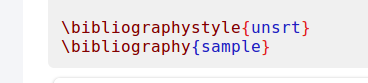
\includegraphics[width=7cm]{bibtexZaseban.png}
    \end{figure}
    \item \textbackslash bibliographystyle\{unsrt\} - stil izgleda teksta kao u dokumentu \\
    \item \textbackslash bibliography\{sample\} - uključivanje \textbf{sample.bib} (BibTeX) datoteke \\
\end{itemize}    
\end{frame}

\begin{frame}
\begin{itemize}
    \item primjer \textbf{.bib} datoteke:
    \begin{figure}
    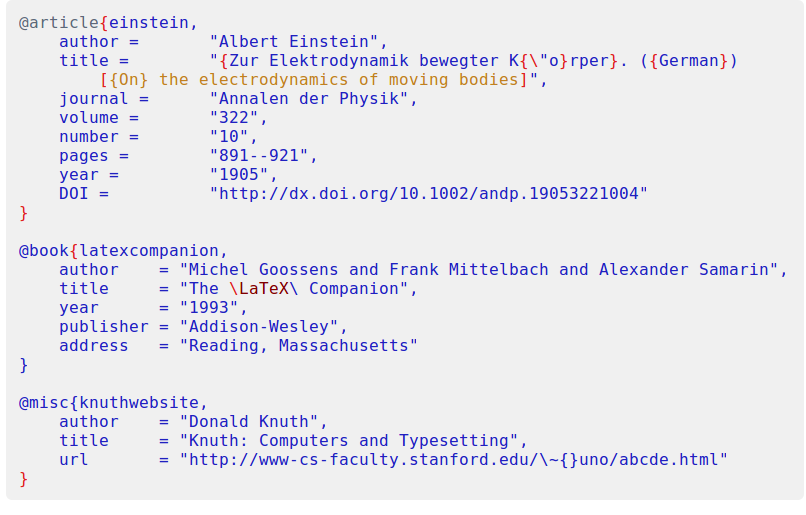
\includegraphics[width=10cm]{bibtexZaseban2.png}
    \end{figure}
\end{itemize}    
\end{frame}

\begin{frame}
Objašnjenje naredbi:
\begin{itemize}
    \item @(article,book,online,misc...) - vrsta reference \\
    \item \{\textbf{ime} ..... - početak i ime reference \\
    \item podatci o: autoru, naslovu, godini... \\
    \item \} - kraj reference
\end{itemize}
Dodavanje bibliografije tablici sadržaja:
\begin{itemize}
    \item Ručno: \\
    \begin{itemize}
        \item \textbackslash addcontentsline \{toc\}\{chapter\}\{Bibliography\} - za knjige \\
        \item \textbackslash addcontentsline \{toc\}\{section\}\{References\} - za članke \\
    \end{itemize}
    \item Automatski: \textbackslash usepackage[nottoc]\{tocbibind\} - sam prepoznaje namjenu\\
\end{itemize}
\end{frame}

\begin{frame}{Natbib\cite{natbib}}
\section{Natbib}
\begin{itemize}
	\item jedan od paketa za upravljanje bibloigrafijama \\
	\item stabilan i vrlo često korišten \\
	\item primjer korištenja: \\ 
	\begin{figure}
	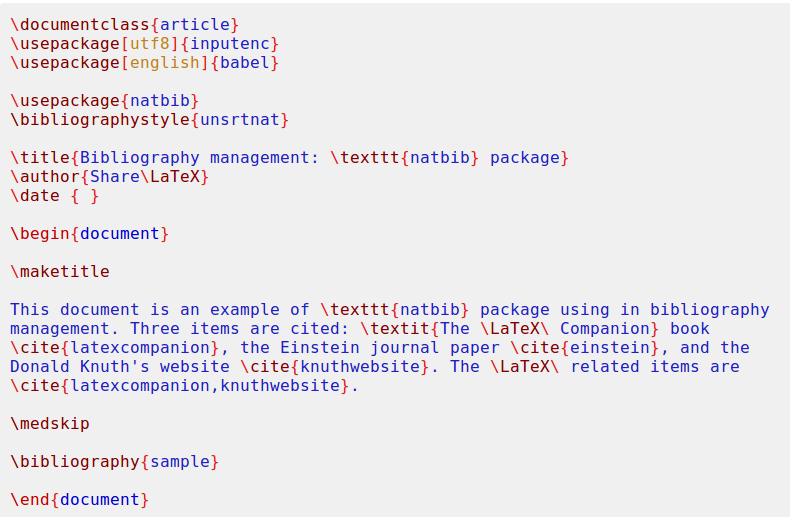
\includegraphics[width=5cm]{natbibprimjer.png}
	\end{figure}
\end{itemize}
\end{frame}

\begin{frame}
\begin{itemize}
	\item paket se poziva naredbom \textbackslash usepackage\{natbib\}\\
	\item i ovdje se koristi naredba \textbackslash cite ali dorađena\\
	\begin{itemize}
		\item \textbackslash citet za tekstualne izvore \\
		\item \textbackslash citeyear za godine itd. \\
	\end{itemize}  
	\item naredbom \textbacklash bibliography{sample} učitati će se datoteka sample.bib \\
	\item sample.bib sadrži izvore bibliografije \\
\end{itemize}
\end{frame}

\begin{frame}{Natbib i sintaksa}
\subsection{Natbib i sintaksa}
\begin{itemize}
	\item koristi se već spomenuta Bibtex sintaksa \\
	\item nakon znaka @ se navodi na što se informacija u referenci odnosi \\
	\begin{itemize}
		\item @article\{...\} \\
		\item @book \{...\}\\
		\item @online \{...\} ... \\
	\end{itemize}
	\item primjer navođenja internetskih stranica \\
		\begin{itemize}
			\item author = Ime autora \\
			\item title = Naziv članka \\
			\item url = "http://www.onlinečlanak.com" \\
		\end{itemize}
\end{itemize}
\end{frame}

\begin{frame}{Dodatne opcije}
\begin{itemize}
	\item dodaju se unutar uglatih zagrada i odvajaju se zarezom \\
	\item njima se mijenja pozadina, stil (redoslijed referenci), način sortiranja... \\
	\item primjeri:
	\begin{itemize}
			\item square - koristi uglate zagrade \\
			\item numbers - za numerička citiranja \\
			\item comma - odvaja citate zarezom \\
			\item longnamefirst - prvo navodi cijelo ime autora \\
	\end{itemize}
\end{itemize}
\end{frame}

\begin{frame}{Dodavanje bibliografije u sadržaj}
\subsection{Dodavanje biblografije u sadržaj}
\begin{itemize}
	\item da bi se bibliografija uključila u tablicu sadržaja uvodi se paket tocbibind \\
	\item dodatne opcije se upisuju pokraj \textbackslash printbibliography \\
	\item primjer:
	\begin{figure}
	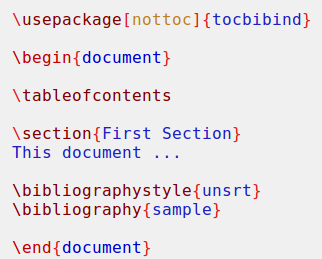
\includegraphics[width=5cm]{natbibprimjer2.png}
	\end{figure}
\end{itemize}
\end{frame}

\begin{frame}{Stilovi bibliografija}
\begin{itemize}
	\item primjer navođenja izabranog stila: \\
	\begin{figure}
	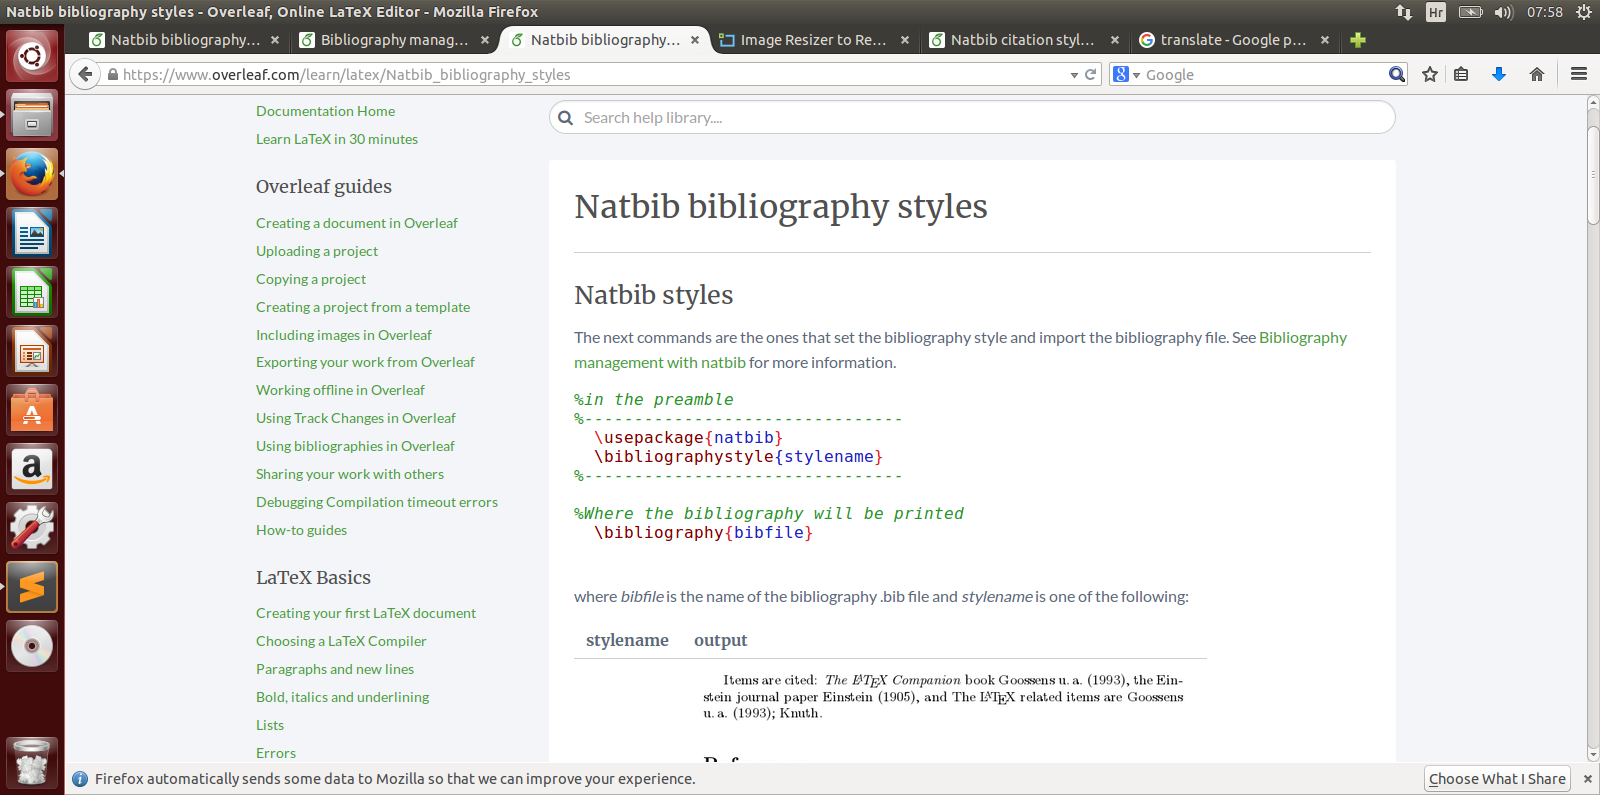
\includegraphics[width=5cm]{natbibprimjer3.png}
	\end{figure}
	\item neki stilovi su:
	\begin{itemize}
			\item dinat, humannat, plainnat, abbrvnat itd.  \\
	\end{itemize}
\end{itemize}
\end{frame}


\begin{frame}{Alati za vođenje bibliografije}
\section{Alati za vođenje bibliografije}
Neki od alata za vođenje bibliografija:
 \begin{itemize}
	\item Mandeley \\
	\item JabRef \\
	\item ReadCube \\
	\item Zotero \\
\end{itemize}
 \end{frame}

 

\begin{frame}{Mandeley}
\subsection{Mandeley}
\begin{itemize}
	\item besplatni softver tvrtke Elsevier \\
	\item koristan za upravljanje i razmjenu znanstvenih radova \\
	\item može upravljati bibliografijom u Open Officeu i čitati BibTeX \\
	\item mogu se pronaći  tuđe .bib datoteke na web-stranici relevantne za  
	određene teme (copy – paste i vlastiti .bib je spreman) \\
\end{itemize}
 \end{frame}

 

\begin{frame}{JabRef}
\subsection{JabRef}
\begin{itemize}
	\item Java program (pod GPL licencom) \\
	\item omogućuje pretraživanje mnogih bibliografskih baza i upravljanje
	BibTeX lokalnim bazama  \\
	\item može izvesti podatke u različitim izlaznim formatima (HTML, MS Word, EndNote…) \\
\end{itemize}
 \end{frame}

 
\begin{frame}{Zotero}
\subsection{Zotero}
\begin{itemize}
	\item najjednostavniji za korištenje  \\
	\item besplatna i samostalna aplikacija za uvoz i izvoz datoteka \\
	\item ima posebne dodatke za preglednike Chrome i Firefox \\
	\item uz podršku za više od 9000 stilova citiranja, omogućuje oblikovanje
	 rada u bilo kojem stilu i izdanju \\
\end{itemize}
\end{frame}


\begin{frame}{Zaključak}
\section{Zaključak}
\begin{itemize}
	\item jedna od velikih prednosti LaTex-a je jednostavno manipuliranje bibliografijama \\
	\item bibtex je osnovni paket te je i najjednostavniji \\
	\item biblatex pruža više mogućnosti konfiguracije i više stilova \\
	\item natbib omogućava najviše stilova prikaza literature pa je i najkompliciraniji za korištenje \\
\end{itemize}
\end{frame}

\begin{frame}
\printbibliography[title={Literatura}]
\end{frame}

\begin{frame}
Hvala na pažnji!
\end{frame}

\end{document}